\documentclass{article}
\usepackage[T1]{fontenc}
\usepackage{lmodern}
\usepackage{graphicx}
\usepackage{amsmath,amssymb}
\usepackage[a4paper,margin=2cm]{geometry}
\usepackage[absolute,overlay]{textpos}
\setlength{\TPHorizModule}{1mm}
\setlength{\TPVertModule}{1mm}
\usepackage[indonesian]{babel}
\usepackage{hyperref}
\setlength{\emergencystretch}{2em}
% unit: Halaman 70

\begin{document}

% === Halaman 70 (llm) ===

\section*{B. Program ekstraksi pesan}

\vspace{252.45mm}

\begin{verbatim}
% Nama file: LSB_estrak.m
% Ekstraksi pesan dari citra stegano dengan metode modifikasi LSB. Panjang
% pesan (L) telah disimpan di dalam citra stegano.
% Asumsi: jumlah bit untuk merepresentasikan panjang pesan maksimal 30 bit.
% Input: Citra stegano (berwarna)
% Output: pesan (teks)
% Diprogram oleh Rinaldi Munir, @Informatika STEI-ITB

clear all;

% Baca citra stegano
namaFile = input('Ketikkan nama file citra stego: ', 's');
stegoImage = imread(namaFile);
imshow(namaFile); title ('Citra stego ');

% Ekstraksi bit-bit panjang pesan terlebih dahulu
% Diperlukan 30 byte = 10 pixel x 3 byte pada baris pertama citra stegano
idx = 1;
for col = 1:10
    for i = 1:3
        nL(idx) = bitget(stegoImage(1,col, i), 1);
        idx = idx + 1;
    end
end
\end{verbatim}

% deskripsi: Screenshot potongan kode MATLAB untuk program ekstraksi pesan menggunakan metode LSB.
% bbox normalisasi: [0.0500, 0.1100, 0.8000, 0.9600]
\begin{textblock*}{157.50mm}(10.50mm,32.67mm)
\noindent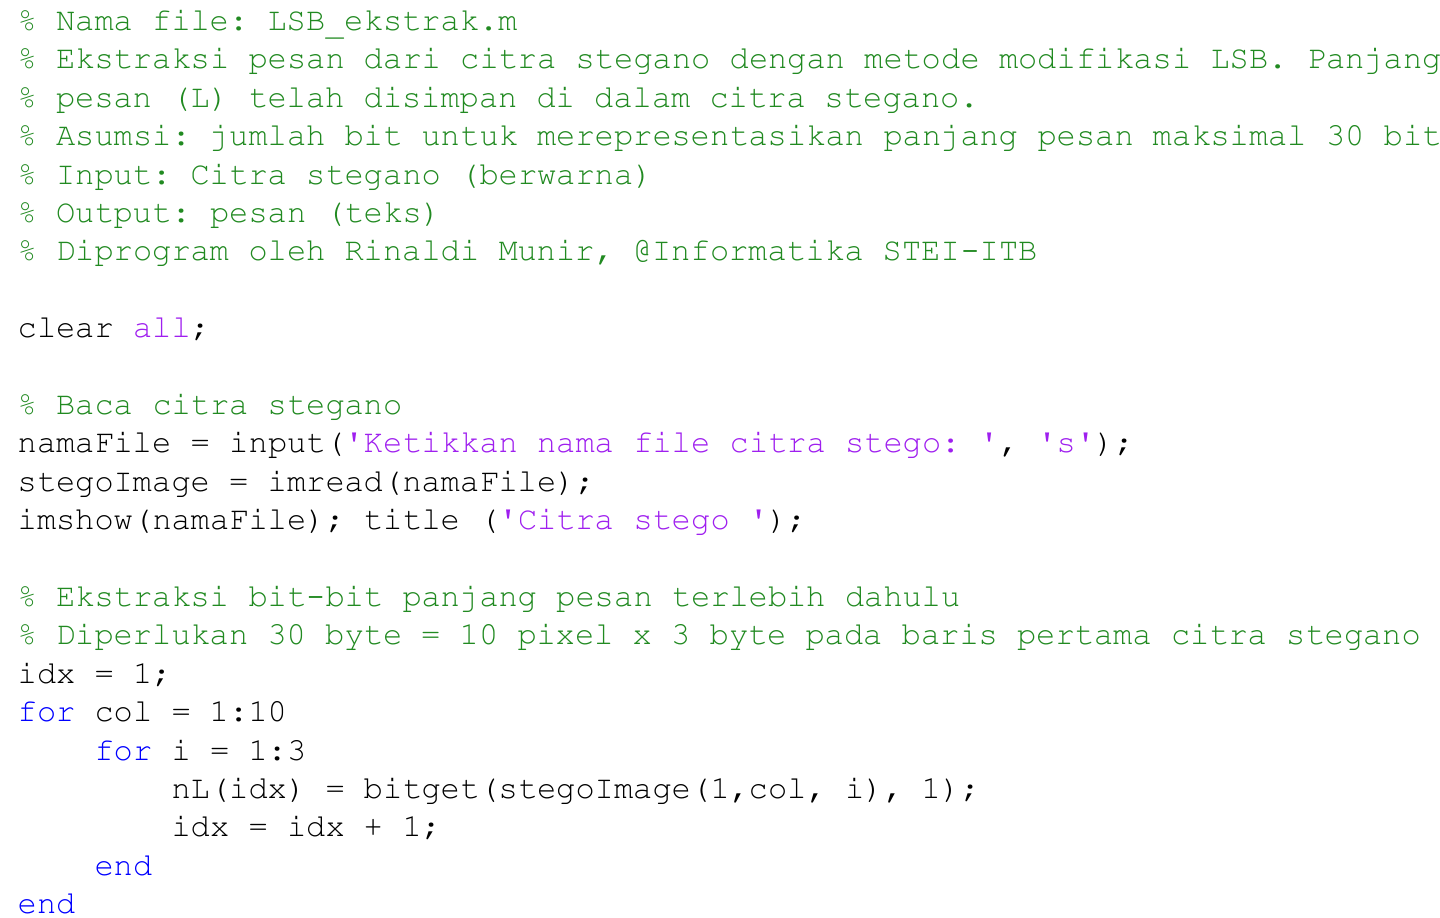
\includegraphics[width=157.50mm,height=252.45mm]{../../images/llm/page_070_img_01.png}%
\end{textblock*}

\end{document}
